\documentclass[10pt]{beamer}

\usepackage[brazilian]{babel}
\usepackage[utf8]{inputenc}
\usepackage[T1]{fontenc}
\usepackage{listings}
\usepackage{microtype}
\usepackage{graphicx}
\usepackage[utf8]{inputenc}
\usepackage[T1]{fontenc}
\usepackage{helvet}

\usetheme[left]{Madrid}
% colored hyperlinks
\newcommand{\chref}[2]{%
  \href{#1}{{\usebeamercolor[bg]{AAUsidebar}#2}}%
}

\title[Java SWING]% optional, use only with long paper titles
{\textbf{Java SWING}}

\subtitle{MATA55 - Programação Orientada a Objetos}  % could also be a conference name

\author[Frederico Durão] % optional, use only with lots of authors
{
  Profº Frederico Durão\\
  \href{mailto:freddurao@dcc.ufba.br}{{\tt freddurao@dcc.ufba.br}}
}

\institute[
 % {
\includegraphics[scale=0.2]{AAUgraphics/logodcc}}\\ %insert a company, department or university logo
 Dept.\ de Ciência da Computação\\
 % UFBA\\

] % optional - is placed in the bottom of the sidebar on every slide
{% is placed on the title page
  Instituto de Matemática\\
  Departamento de Ciência da Computação\\
  Universidade Federal da Bahia\\

  
  %there must be an empty line above this line - otherwise some unwanted space is added between the university and the country (I do not know why;( )
}


% specify a logo on the titlepage (you can specify additional logos an include them in 
% institute command below
\pgfdeclareimage[height=3cm]{titlepagelogo}{AAUgraphics/aau_logo_new} % placed on the title page
%\pgfdeclareimage[height=1.5cm]{titlepagelogo2}{graphics/aau_logo_new} % placed on the title page
\titlegraphic{% is placed on the bottom of the title page
  \pgfuseimage{titlepagelogo}
%  \hspace{1cm}\pgfuseimage{titlepagelogo2}
}

% Formatação dos trechos em Java
\definecolor{dkgreen}{rgb}{0,0.6,0}
\definecolor{gray}{rgb}{0.5,0.5,0.5}
\definecolor{mauve}{rgb}{0.58,0,0.82}

\lstset{frame=tb,
  language=Java,
  aboveskip=3mm,
  belowskip=3mm,
  showstringspaces=false,
  columns=flexible,
  basicstyle={\small\ttfamily},
  numbers=none,
  numberstyle=\tiny\color{gray},
  keywordstyle=\color{blue},
  commentstyle=\color{dkgreen},
  stringstyle=\color{mauve},
  breaklines=true,
  breakatwhitespace=true
  tabsize=3
}
%Formatação dos trechos em java acabam aqui.


\graphicspath{{images/}}
\begin{document}
% the titlepage
{
\begin{frame}[plain,noframenumbering] % the plain option removes the sidebar and header from the title page
  \titlepage
\end{frame}}
%%%%%%%%%%%%%%%%

% TOC
\begin{frame}[allowframebreaks]{Agenda}{}
\tableofcontents{}
\end{frame}
%%%%%%%%%%%%%%%%

\section{Introdução}
\subsection{O que é Java Swing}
\begin{frame}{Introdução}{O que é Java Swing}
\begin{itemize}
\item Swing é uma API Java para interfaces gráficas. 
\item Faz parte da JFC (Java Foundation Classes) que encapsula um grupo de 'features' para GUIs (Graphical User Interfaces).
\end{itemize}
\end{frame}
\subsection{Por que estudar Java Swing}
\begin{frame}{Introdução}{Por que estudar Java Swing}
\end{frame}
\subsubsection{Swing vs. others}
\begin{frame}{Introdução}{Por que estudar Java Swing}{Swing vs. others}
\end{frame}
%			EXT-GWT
%			Android
%			JSF + PrimeFaces
%			OpenGL, WebGL
\subsection{Como usar o Java Swing}
\begin{frame}{Introdução}{Como usar o Java Swing}
\begin{itemize}
\item Editor convencional.
\item Plugins Drop \& Drag.
\end{itemize}
\end{frame}{}
\subsubsection{Codificando no Editor convencional}
\begin{frame}[allowframebreaks]{Introdução}{Como usar o Java Swing}{Codificando no Editor convencional}
\lstinputlisting[language=Java]{codes/HelloWorldSwing.java}
\end{frame}{}

\begin{frame}{Introdução}{Como usar o Java Swing}
  \begin{figure}[!htb]
    \centering
    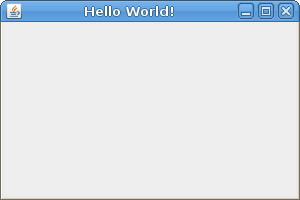
\includegraphics[scale=0.5]{hello_world}
    \caption{HelloWordSwing.java}
    \label{figRotulo}
  \end{figure}
\end{frame}{}


\begin{frame}{Introdução}{Criando Projeto}
  \begin{figure}[!htb]
    \centering
    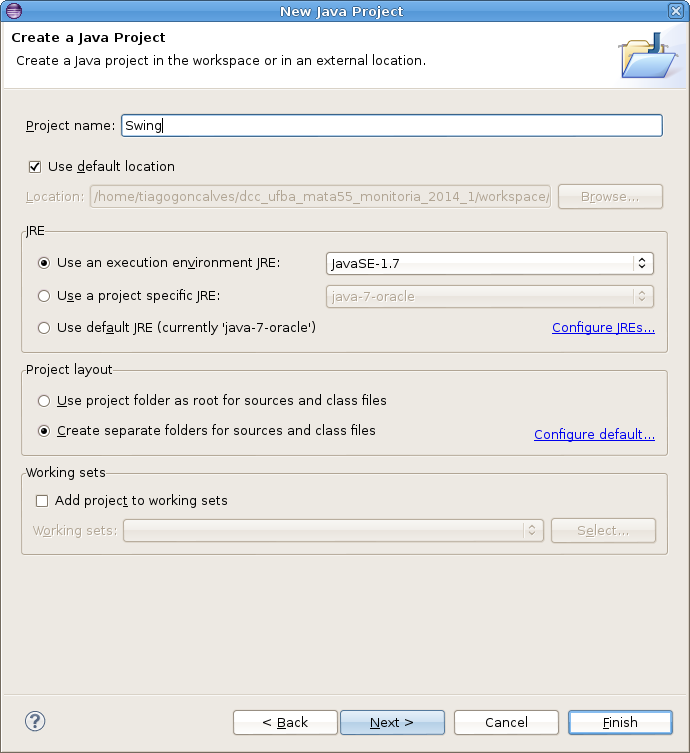
\includegraphics[scale=0.25]{criando_projeto_swing}
    \caption{Projeto Java}
    \label{figRotulo}
  \end{figure}
\end{frame}{}

\begin{frame}{Introdução}{Criando Classe Principal}
  \begin{figure}[!htb]
    \centering
    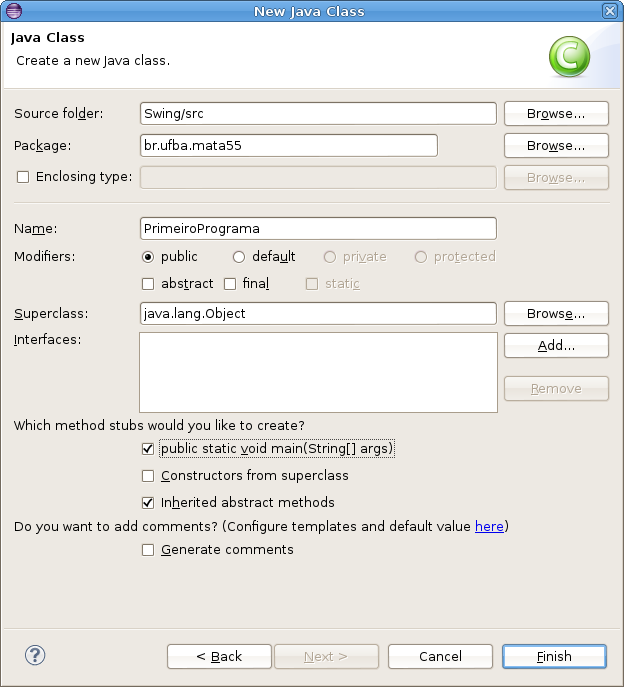
\includegraphics[scale=0.25]{criando_primeiro_programa}
    \caption{PrimeiroPrograma.java}
    \label{figRotulo}
  \end{figure}
\end{frame}{}

\subsubsection{Metodo Drop \& Drag - Plugin WindowBuilder para Eclipse}
\begin{frame}{Página principal do Window Builder para Eclipse}
\textbf{https://www.eclipse.org/windowbuilder/}
  \begin{figure}[!htb]
    \centering
    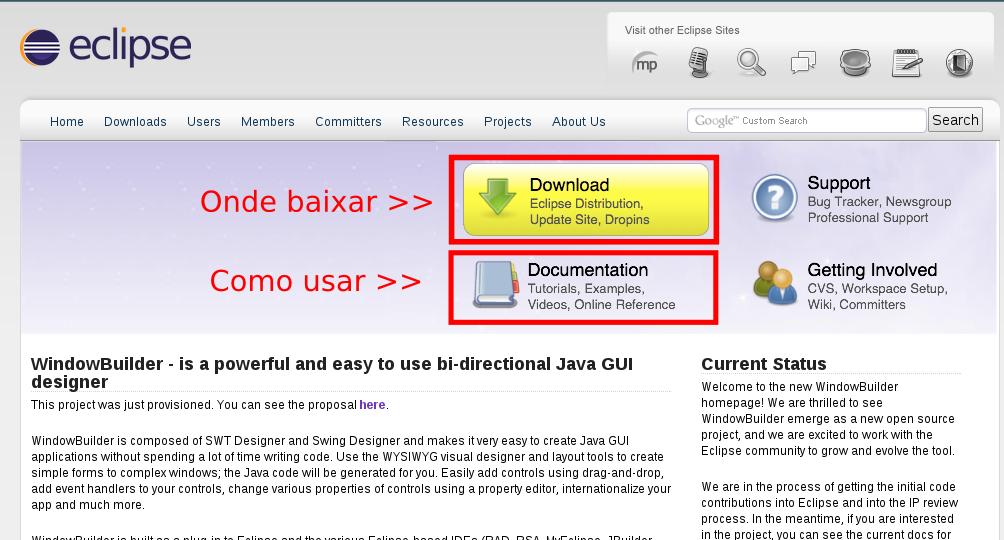
\includegraphics[scale=.4]{pag_principal_window_builder}
    \caption{Página principal do Window Builder}
    \label{figRotulo}
  \end{figure}
\end{frame}{}

\subsubsection{WindowBuilder - Instalando }
\begin{frame}{WindowBuilder - Instalando }
\textbf{Help > Instal New Software}
  \begin{figure}[!htb]
    \centering
    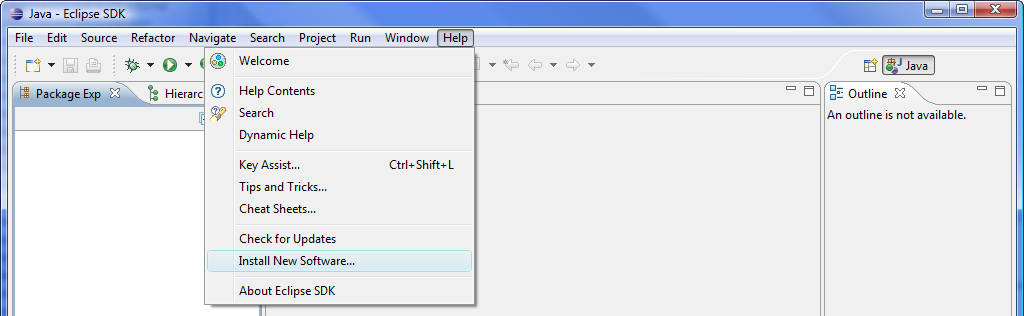
\includegraphics[scale=.4]{instalando_window_builder_1}
    \caption{Instalando Window Builder}
    \label{figRotulo}
  \end{figure}
\end{frame}{}

\begin{frame}{WindowBuilder - Instalando }
Clique em \textbf{Add}.
  \begin{figure}[!htb]
    \centering
    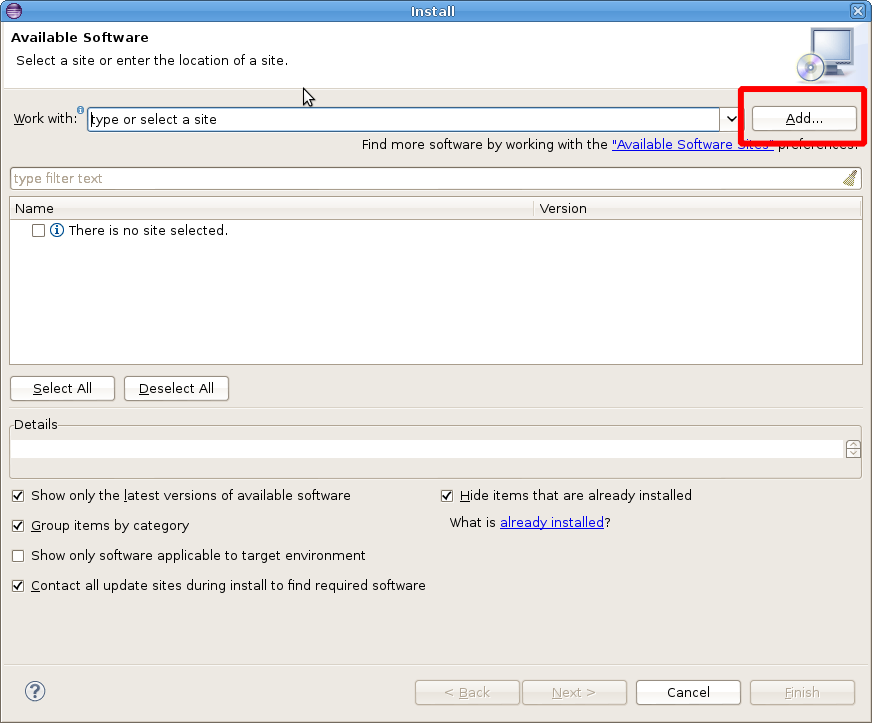
\includegraphics[scale=.3]{window_builder_add}
    \caption{Instalando Window Builder}
    \label{figRotulo}
  \end{figure}
\end{frame}{}

\begin{frame}{WindowBuilder - Instalando }
Em \textbf{Name} digite \textbf{WindowBuilder} (pode ser qualquer nome).
\linebreak
Em \textbf{Location} digite a url 
	http://download.eclipse.org/windowbuilder/WB/release/R201309271200/4.3/
  \begin{figure}[!htb]
    \centering
    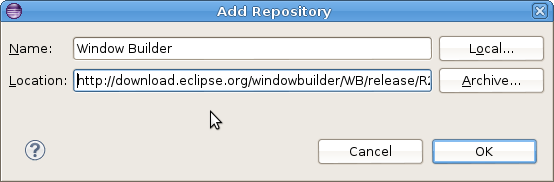
\includegraphics[scale=.3]{window_builder_url}
    \caption{Instalando Window Builder}
    \label{figRotulo}
  \end{figure}
\end{frame}{}

\subsubsection{WindowBuilder - Perspectiva }
\begin{frame}{Abrindo Editor do Window Builder}
Clique com o botão direito na classe PrimeiroPrograma.java . Selecione \textbf{Open with} e depois \textbf{WindowBuilder Editor}.
  \begin{figure}[!htb]
    \centering
    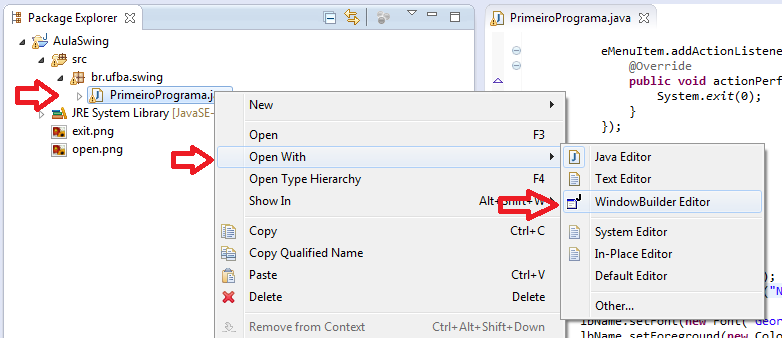
\includegraphics[scale=.4]{window_builder_perspective}
    \caption{Abrindo Editor do Window Builder}
    \label{figRotulo}
  \end{figure}
\end{frame}{}

\begin{frame}{Abrindo Editor do Window Builder}
\begin{itemize}
\item \textbf{Source} - Como o Editor padrão do Eclipse.
\item \textbf{Design} - Editor gráfico do Window Builder.
\end{itemize}
  \begin{figure}[!htb]
    \centering
    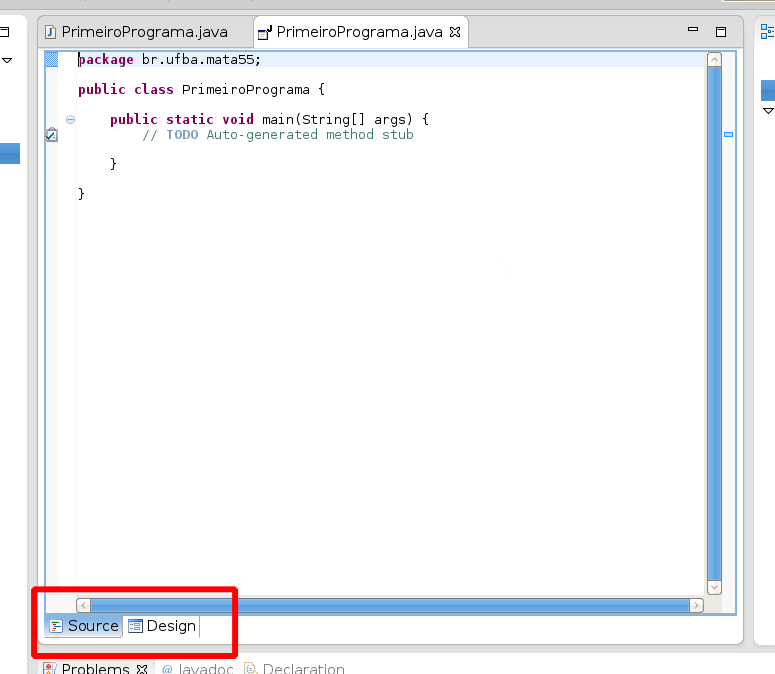
\includegraphics[scale=.3]{windows_builder_perspective_source}
    \caption{Editor do Windows Builder}
    \label{figRotulo}
  \end{figure}
\end{frame}{}

\begin{frame}{Aba Design do Editor do Window Builder}
\begin{itemize}
\item Visualizador gráfico.
\end{itemize}
  \begin{figure}[!htb]
    \centering
    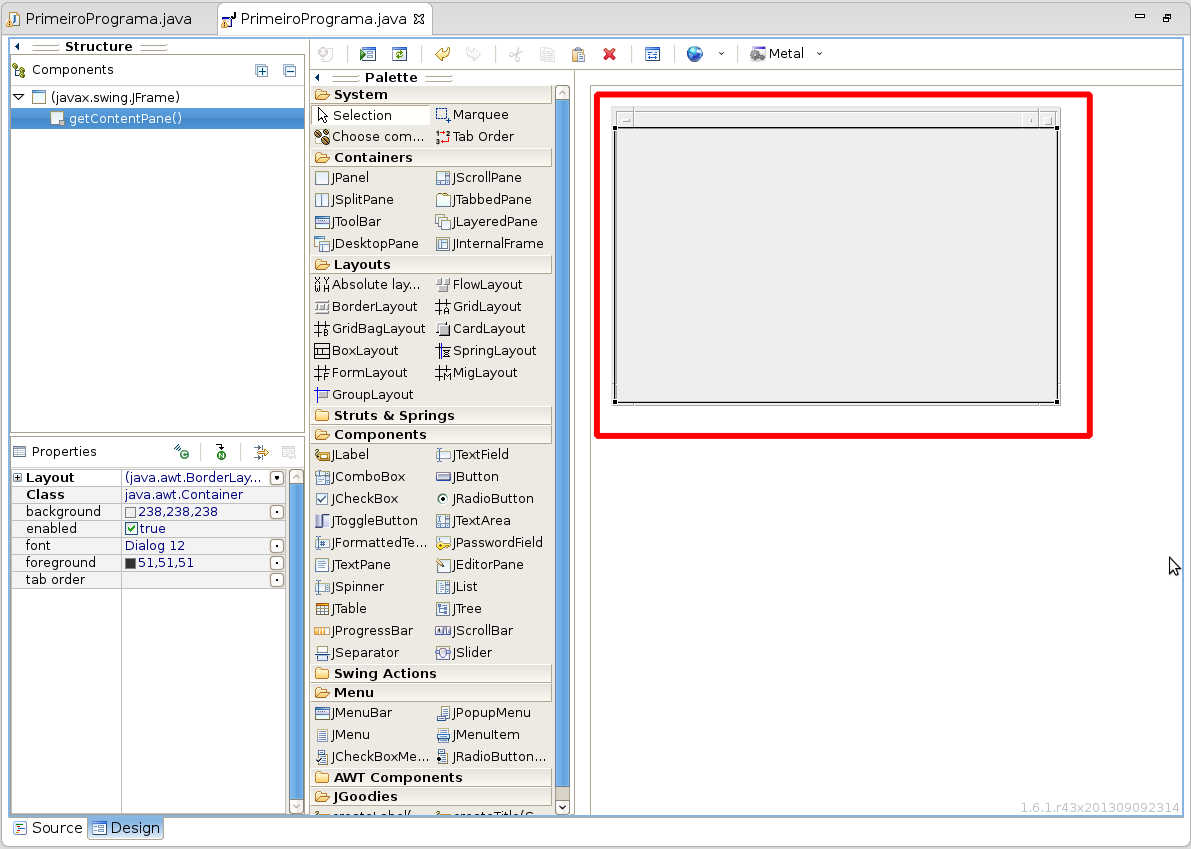
\includegraphics[scale=.25]{windows_builder_perspective_part1}
    \caption{Aba Design}
    \label{figRotulo}
  \end{figure}
\end{frame}{}

\begin{frame}{Aba Design do Editor do Window Builder}
\begin{itemize}
\item \textbf{Structure} - estrutura da tela com seus componentes.
\item \textbf{Properties} - propriedades do componente selecionado.
\end{itemize}
  \begin{figure}[!htb]
    \centering
    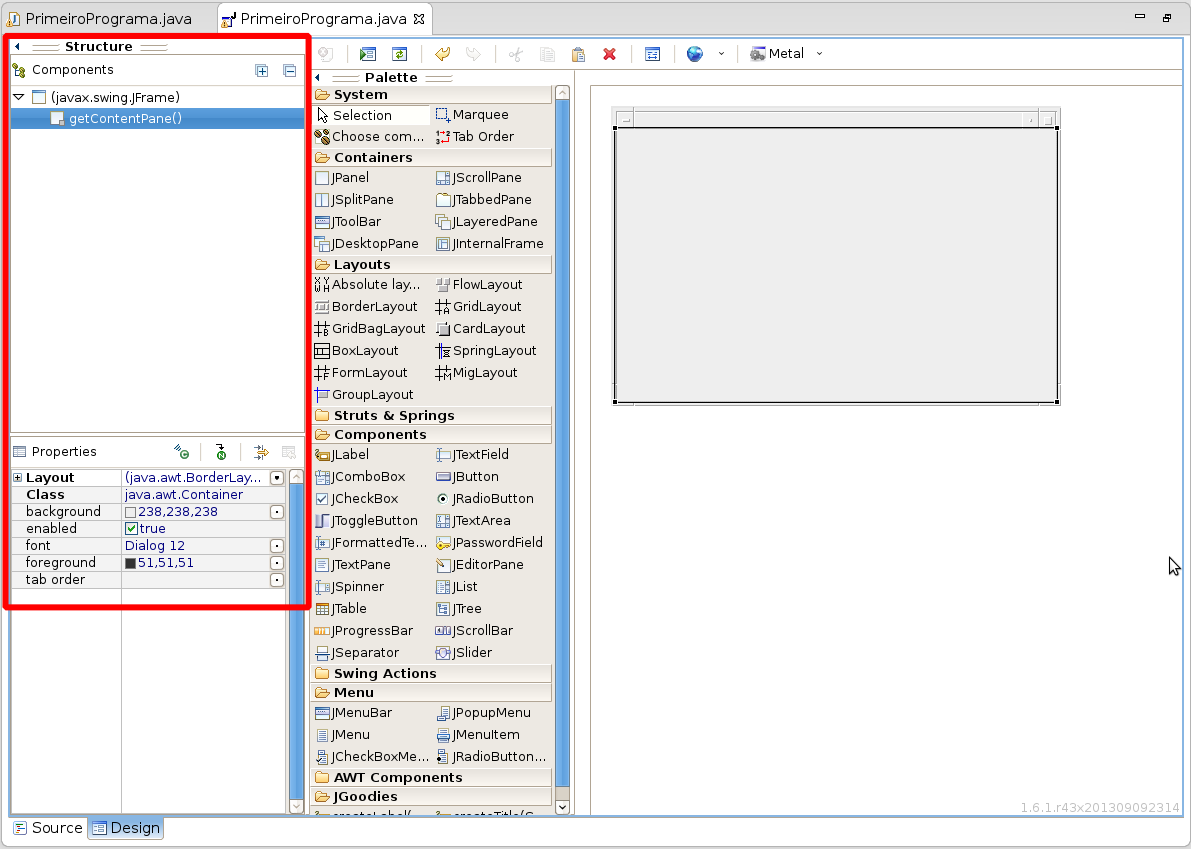
\includegraphics[scale=.25]{windows_builder_perspective_part3}
    \caption{Estrutura e propriedades}
    \label{figRotulo}
  \end{figure}
\end{frame}{}

\begin{frame}{Construindo a janela}
Inserindo um título à janela.
\linebreak
Selecione a janela e insira em \textbf{Title} na aba \textbf{Properties}.
  \begin{figure}[!htb]
    \centering
    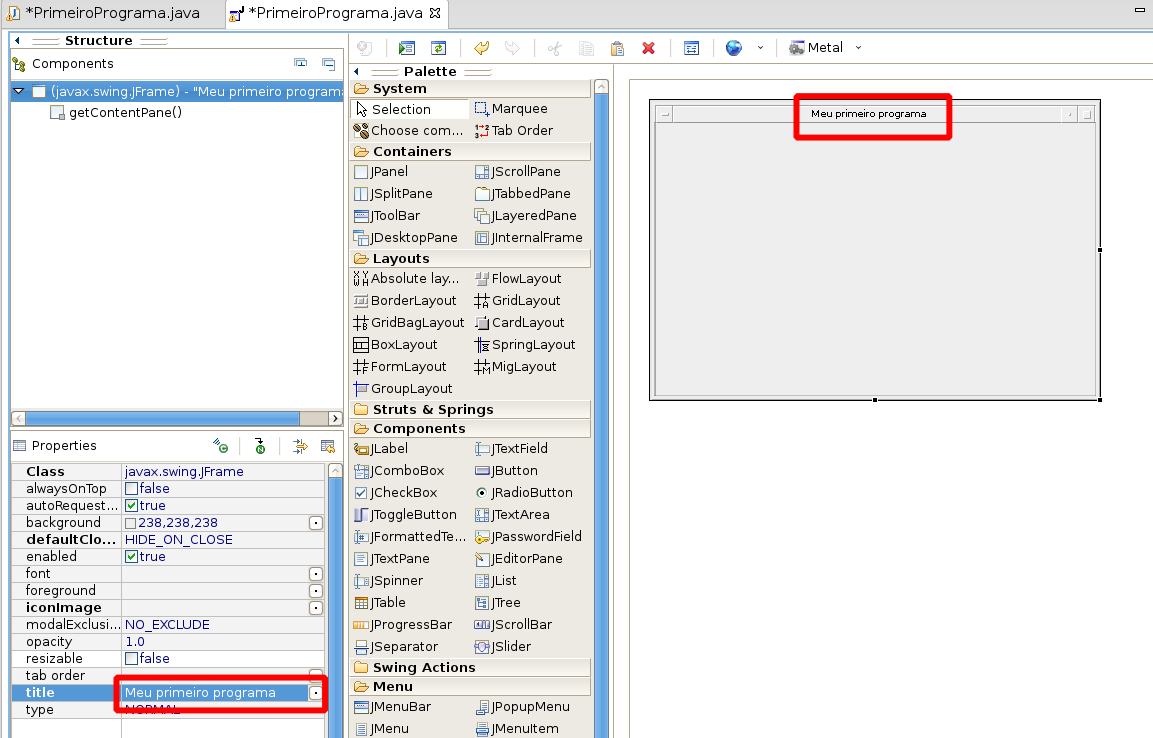
\includegraphics[scale=.3]{colocando_titulo}
    \caption{Estrutura e propriedades}
    \label{figRotulo}
  \end{figure}
\end{frame}{}

\begin{frame}{Construindo a janela}
O equivalente em código seria.
\lstinputlisting[language=Java,linerange=18-19]{codes/PrimeiroPrograma.java}
\end{frame}{}

\begin{frame}{Construindo a janela - \textbf{JPanel}}
%TODO Definição
\end{frame}{}

\begin{frame}{Construindo a janela - \textbf{JPanel}}
\begin{itemize}
\item O Window Builder utiliza o método \textbf{Drag \& Drop} (clica e solta)
\item As áreas verdes são os locais onde o componente pode ser inserido
\item As divisões entre as áreas verdes são ditadas pelo \textbf{layout} escolhido
\item Por padrão o layout é o \textbf{BorderLayout} que divide a tela em \textbf{NORTH}, \textbf{SOUTH},\textbf{WEST}, \textbf{CENTER} e \textbf{EAST}.
\end{itemize}
\begin{figure}[!htb]
    \centering
    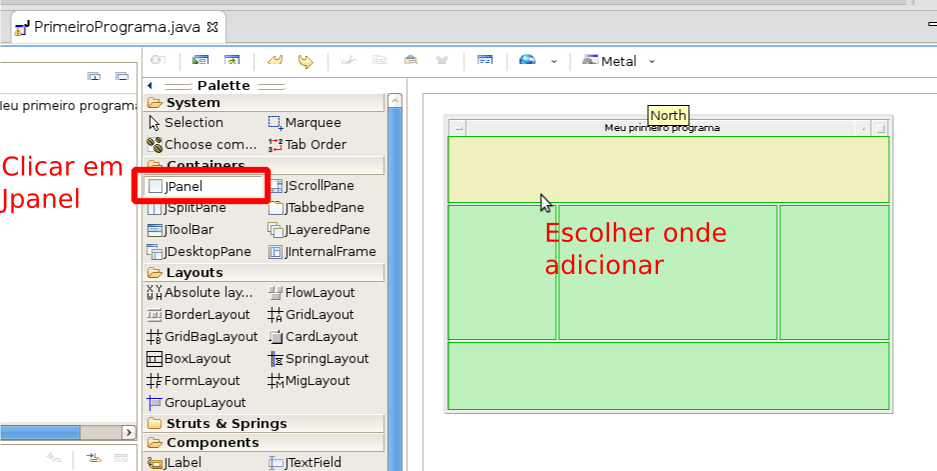
\includegraphics[scale=.4]{jpanel}
    \caption{JPanel}
    \label{figRotulo}
  \end{figure}
\end{frame}{}

\begin{frame}{Construindo a janela - \textbf{JPanel}}
Em código:
\lstinputlisting[language=Java]{codes/PrimeiroProgramaPura.java}
\end{frame}{}

\begin{frame}{Construindo a janela - \textbf{JLabel}}
%TODO Definição
\end{frame}{}


\begin{frame}{Construindo a janela - \textbf{JLabel}}
\begin{itemize}
\item Ao inserir o JLabel já defina o nome!
\end{itemize}
\begin{figure}[!htb]
    \centering
    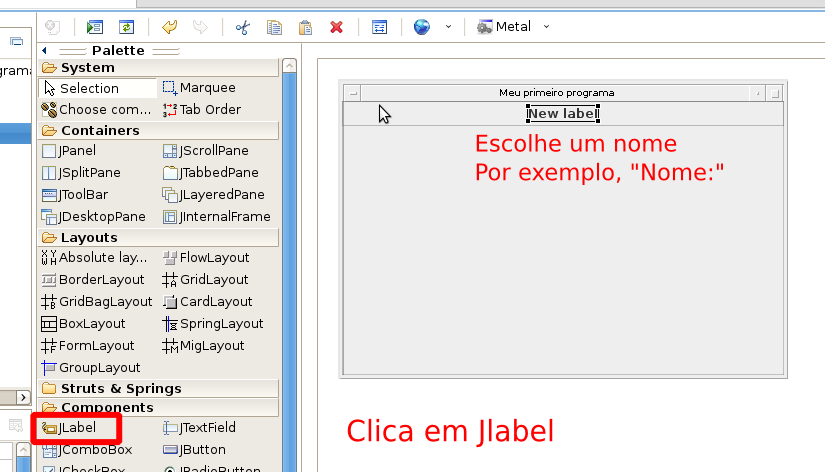
\includegraphics[scale=.4]{jlabel}
    \caption{JLabel}
    \label{figRotulo}
  \end{figure}
\end{frame}{}

\begin{frame}{Construindo a janela - \textbf{JTextField}}
%TODO Definição
\end{frame}{}

\begin{frame}{Construindo a janela - \textbf{JTextField}}
\begin{figure}[!htb]
    \centering
    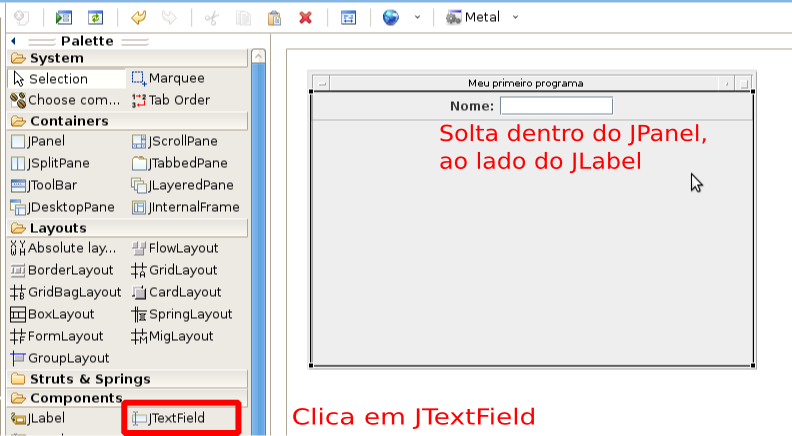
\includegraphics[scale=.4]{jtextfield}
    \caption{JTextField}
    \label{figRotulo}
  \end{figure}
\end{frame}{}

\begin{frame}{Construindo a janela - Alinhando os componentes}
\begin{itemize}
\item Os tipos de alinhamento disponíveis são : \textbf{LEFT}, \textbf{RIGHT}, \textbf{CENTER}, \textbf{LEADING}(bottom) e \textbf{TRAILING} (top)
\end{itemize}
\begin{figure}[!htb]
    \centering
    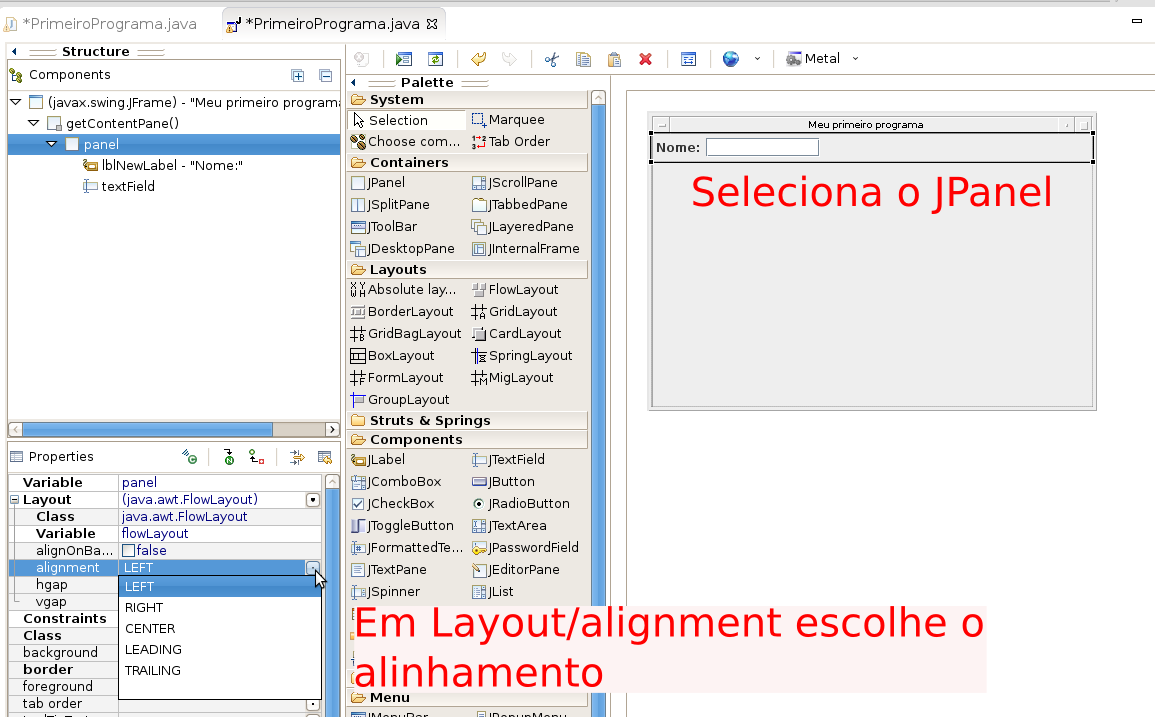
\includegraphics[scale=.25]{alinhando_a_esquerda}
    \caption{Alinhando componentes}
    \label{figRotulo}
  \end{figure}
\end{frame}{}

\begin{frame}{Construindo a janela - \textbf{Alinhamento}}
Em código:
\lstinputlisting[language=Java,linerange=28-38]{codes/PrimeiroPrograma.java}
\end{frame}{}



%%%%%%%%%%%%%%%%%%%%%%%%%%%%%%%%%%%%%%%%%%%%%%%%%%%%%%%%%%%%%%%%%%%%%%%%%
\section{Referências}
\begin{frame}{Referências}{}
\begin{itemize}
\item Window Builder - https://www.eclipse.org/windowbuilder/
\item Swing tutorial - http://www.tutorialspoint.com/swing/
\item Swing tutorial(verboso) - http://www.wikihow.com/Create-a-Swing-GUI-in-Java
\item Swing tuto mais completo - http://zetcode.com/tutorials/javaswingtutorial/
\item Swing oficial - http://docs.oracle.com/javase/tutorial/uiswing/components/
\item Swing oficial - http://docs.oracle.com/javase/tutorial/uiswing/
\item Swing javadoc - http://docs.oracle.com/javase/7/docs/api/javax/swing/package-summary.html
\end{itemize}
\end{frame}
\end{document}